\documentclass[11pt]{article}

\usepackage[margin=2.35cm]{geometry}
\usepackage{amsmath,amssymb,booktabs,array}
\usepackage{graphicx,xcolor,caption,enumitem,placeins}
\usepackage[hidelinks]{hyperref}
\usepackage{tikz}
\usetikzlibrary{arrows.meta,positioning}

\graphicspath{{figures/}}
\setlist[itemize]{topsep=3pt,itemsep=2pt,leftmargin=1.3em}
\setlist[enumerate]{topsep=3pt,itemsep=2pt,leftmargin=1.4em}
\captionsetup{font=small,labelfont=bf,skip=6pt}
\setlength{\parskip}{5pt}
\setlength{\parindent}{0pt}

\definecolor{navy}{HTML}{1F4E79}
\definecolor{rule}{HTML}{D0D5DD}

\pagestyle{plain}
\newcommand{\modelid}{OM-V9}
\newcommand{\doctype}{Model Development Document}

\title{\textcolor{navy}{\doctype}\\[4pt]
\large Off-market automated valuation, version 9}
\author{Model identification: \modelid}
\date{7 November 2026}

\begin{document}
\maketitle
\thispagestyle{empty}

\begin{center}
\small
\begin{tabular}{@{}>{\bfseries}l p{11.2cm}@{}}
Track & Off-market valuation, before a home is listed \\
Status & Development candidate, pending independent validation \\
Population & Synthetic Toronto listings, sales closed January 2021--May 2026 \\
Decision metric & Median absolute percentage error (MdAPE) on sold price \\
Performance claim & Walk-forward MdAPE \(7.45\%\), MAPE \(9.79\%\), median bias \(-0.37\%\) \\
Benchmark & 12-month community \$/sqft anchor, same sales: MdAPE \(15.33\%\) \\
Source notebook & \texttt{off\_market\_models.ipynb} \\
Submission code & \texttt{features.py}, \texttt{models.py}, \texttt{run.py} \\
Figure reproduction & \texttt{model-report/reproduce\_v9\_figures.py} \\
\end{tabular}
\end{center}

\vspace{4pt}
{\color{rule}\hrule}
\vspace{8pt}

\section*{How to read this document}

This is the development record for \modelid, the off-market model. It values a home that has no asking price. It is the companion to the list-aware document for LA-V22. The two must not be quoted as if they answered the same question. LA-V22 sees the ask and reaches a walk-forward MdAPE of \(4.28\%\). This model does not see the ask, and its walk-forward MdAPE is \(7.45\%\).

Two results are kept apart.

\begin{itemize}
\item \textbf{Developmental score.} One fit on every sale that closed before December 2025, scored on the 10,069 sales from December 2025 through May 2026. For the adopted \modelid{} specification this is MdAPE \(7.53\%\).
\item \textbf{Walk-forward score.} The same six months, each predicted by a model fit only on sales that had already closed. This is the performance claim: MdAPE \(7.45\%\).
\end{itemize}

The walk-forward number is the one a validation team should sign against. Segmented charts come from a fresh developmental refit. That refit reproduced the notebook to the reported precision (MdAPE \(7.53\%\), MAPE \(9.77\%\), median signed error \(-2.10\%\)).

\tableofcontents
\newpage

\section{Purpose and intended use}
\label{sec:purpose}

\subsection{The decision}

The question is what a home is worth before anyone has published an asking price. A lender marking collateral, or a desk screening a property that is not yet listed, does not have the quote that carries most of the list-aware model. \modelid{} returns a point estimate of the sold price from the physical description, the location, the words in a description, and sales that have already closed.

List price is on the historical sales file. It is not an input. The off-market test file does not have it, and a model that used it would be answering the list-aware question with an off-market label.

\subsection{What the model returns}

\[
\hat Y_i = \exp\bigl(F(x_i)\bigr)\,\exp(-w\,\delta),
\]
with \(w = 1\). \(F\) is a gradient-boosted tree on log sold price. \(\delta\) is a level correction: the median log miss of an earlier tree, measured on the three months before the scoring origin and applied as a common percent. There is no prediction interval and no recommended haircut beyond this one correction. The correction is part of the specification, not an overlay a user is invited to change.

\subsection{Users and non-uses}

The intended user is an internal valuation function that cannot see an ask. The specification is implemented as \texttt{OffMarketModel} in \texttt{models.py}. \texttt{run.py} fits it, runs the walk-forward, and writes the test-file submission. Section~\ref{sec:repro} is that path. \texttt{NearestSalesBaseline} is still in the file and is not the model the pipeline calls.

The model is not an appraisal. It should not be fed list price, days on market, or the third-party AVM. Days on market are known only after the sale. The AVM is absent from the test file, and its date on the training file can fall after the sale.

\subsection{Performance claim, stated once}

On the 10,069 sales closed from December 2025 through May 2026, with each month scored by a refit that could not see that month:

\begin{center}
\begin{tabular}{lrrr}
\toprule
 & MdAPE & MAPE & Median signed error \\
\midrule
12-month community \$/sqft (V1) & 15.33\% & 20.32\% & \(+3.19\%\) \\
\modelid{} walk-forward & 7.45\% & 9.79\% & \(-0.37\%\) \\
\bottomrule
\end{tabular}
\end{center}

MdAPE falls by \(7.88\) percentage points relative to pricing the home at its recent community dollars per square foot, a \(51\%\) reduction. The pooled median bias is about \(0.4\%\) low. That pool hides a month that is \(4.4\%\) low and a month that is \(1.7\%\) high. Section~\ref{sec:walk} is the place to read the bias. The project handout's simple baseline, the median sale of the same type in the same neighbourhood over the previous 12 months, is \(17.7\%\) MdAPE on this window. The starter nearest-ten-sales model is \(20.8\%\). Those two numbers were not refit for this document. They are the published bars this track has to clear, and \modelid{} clears both.

\section{Conceptual soundness}
\label{sec:concept}

\subsection{Economic object}

Without an ask, the model has to produce the price level itself. The hedonic idea (Rosen, 1974) is that a home's price is a function of its attributes and of what similar homes have just sold for. Here the attributes are size, lot, rooms, type, style, and location. The market is the recent sold price per square foot in the same community and type, a citywide price, and earlier sales at the same coordinates.

A useful benchmark is the community anchor
\[
A_i = S_i \times m_{c(i), t(i)}(\tau_i),
\]
where \(S_i\) is square feet, \(\tau_i\) is the listing month, and \(m\) is the median sold dollars per square foot of the same community and type over the 12 months before \(\tau_i\). Fewer than 30 sales falls back to the type, then to the city. On the developmental window this anchor has MdAPE \(15.60\%\). It is a serious model. It is also biased high by \(3.7\%\), because a 12-month median lags a market that has moved, and because one dollars-per-foot number ignores rooms, lot, condition language, and the particular building.

\subsection{Why log price, and why not only a gap around the anchor}

Sold prices run from about \(\$173{,}000\) to \(\$30\) million. Skew of the dollar price is \(5.04\); skew of the log is \(0.80\). A log target makes a unit of error closer to a percent, which is what MdAPE measures.

Versions 3 through 8 fit
\[
g_i = \log(Y_i / A_i)
\]
and reconstruct \(\hat Y_i = A_i \exp(\hat g_i)\). That is the right structure when the anchor is trustworthy and the tree only has to explain the residual. It is the wrong structure when the anchor is stale or the home is unlike the sales that formed it: every error in \(A_i\) is multiplied into the price. \modelid{} predicts \(\log Y_i\) directly. The community price, the city prices, and a building-level price are features, not a base the prediction is forced to start from. The tree can lean on them and can ignore them.

The loss is squared error on the log price,
\[
\sum_i \bigl(\log Y_i - F(x_i)\bigr)^2.
\]
Squared log error is a smooth proxy for percentage error. It is not MdAPE. Exponentiating \(F(x)\) targets a conditional median of a roughly symmetric log residual, which matches a median percentage metric. No smearing correction is applied. A quantile loss aimed at the median directly was tested on the gap specification and did not beat this squared-error direct model (Section~\ref{sec:challengers}).

\subsection{Why a separate level correction}

A tree fit on a long history learns the average level of that history. The last few months can sit above or below it. \(\delta\) is the median of \(\log\hat Y - \log Y\) on the three closed months before the origin, from a tree that was not fit on those three months. Multiplying by \(\exp(-\delta)\) removes that recent median miss. The weight on \(\delta\) was chosen on July--November 2025. Full weight won. A partial weight left more of the bias in place.

This is a second stage. It is one number for every home. It cannot fix a bias that runs in opposite directions at the cheap end and the expensive end. Section~\ref{sec:errors} shows that pattern. The stage is kept because, without it, the July--November error was worse, and because the walk-forward pool is close to unbiased. It is not a claim that every month and every price band is unbiased.

\subsection{Why the evidence has to be out of time}

Community prices, building comps, the remarks score, and \(\delta\) are all computed from other sales. A random split lets them see the future. The rule is the same as in the list-aware document: every table, every category level, every text fit, and every tree uses sales that closed before the home being scored. A building comp has a tighter rule still. It must have closed before the home was listed, and the home's own listing number is removed. Walk-forward validation applies the rule one month at a time.

\section{Data}
\label{sec:data}

\subsection{Source and population}

The sales file is the same synthetic book used for LA-V22. Names, streets, and coordinates do not line up with real maps. No external series is joined.

\begin{center}
\begin{tabular}{llrr}
\toprule
File & Role & Rows & Dates \\
\midrule
\texttt{listings} & Estimation and validation & 150{,}000 & Sold 1 Jan 2021 -- 31 May 2026 \\
\texttt{test\_off\_market} & Unlabelled deployment book & 3{,}974 & Listed 1 Aug 2025 -- 28 Sep 2026 \\
\bottomrule
\end{tabular}
\end{center}

The test file has no sold price and no list price. It is not used to fit, tune, or score anything here. Validation uses the 10,069 closed sales from December 2025 through May 2026, the same homes as the list-aware document, with the ask withheld from the feature set.

\subsection{Estimation sample and the inner slice}

\begin{center}
\begin{tabular}{lrrl}
\toprule
Sample & Rows & Sold from & Sold through \\
\midrule
Developmental estimation & 139{,}931 & 1 Jan 2021 & 30 Nov 2025 \\
Developmental validation & 10{,}069 & 1 Dec 2025 & 31 May 2026 \\
\bottomrule
\end{tabular}
\end{center}

Choices of window, phrases, building specification, remarks score, and shift weight were made on sales from July through November 2025. The model for that screen was fit on sales through June 2025, and the shift inside the screen was measured on April through June from a fit that stopped at the end of March. Those months then go back into the developmental estimation sample. That reuse is why the walk-forward number, which never scores a month the tree has seen, is the claim.

\subsection{Book composition}

Six property types. On the estimation sample the shares are condo apartment \(51.1\%\), detached \(28.6\%\), semi-detached \(9.5\%\), condo townhouse \(6.8\%\), freehold townhouse \(3.4\%\), and co-op apartment \(0.5\%\). There are 5 municipalities, 145 communities, and 16 styles. Training sold-price median \(\$856{,}650\), mean \(\$1{,}073{,}917\), maximum \(\$30{,}000{,}000\).

\subsection{Fields the model is allowed to see}

\begin{center}
\small
\begin{tabular}{llp{6.4cm}}
\toprule
Group & Columns & Treatment \\
\midrule
Timing & date listed & Month enters the seasonal pair; comps must predate it \\
Size & area, beds, baths, parking, garage & Area parsed to square feet; counts kept \\
Lot & lot front, lot depth & Missing when there is no lot \\
Structure & type, style & Categorical, levels frozen on past sales \\
Place & municipality, community, lat, lon & Community is categorical; a pin is lat, lon, and type \\
Text & remarks & Phrase flags, plus a ridge score on word pairs \\
\bottomrule
\end{tabular}
\end{center}

List price is present on the historical sales and is unused. Using it would convert this model into a list-aware model.

\section{Data preparation}
\label{sec:clean}

We keep every sale. Nothing in this section is a filter. The work is turning the raw listing into columns a tree can split on, and keeping a record of what was missing. A few columns are just a cleaned version of a field that arrived as text. The rest are built from other homes, and those are the ones that leak the future if we get the dates wrong. We build those in Section~\ref{sec:features}, after the raw fields are in shape. The level correction, which is a second pass rather than a column, is in Section~\ref{sec:calibration}.

\subsection{The order we run}

\begin{enumerate}
\item Parse \texttt{house\_area} into a square-footage number \(S_i\). Every price-per-foot feature later divides by this.
\item Encode the lot, and leave bedrooms, washrooms, parking, garage, latitude, and longitude as recorded.
\item Build a building pin from the rounded coordinates and the property type. We use the pin only to find earlier sales of the same building.
\item Add a sine and a cosine of the listing month, so December sits next to January.
\item From sales that have already closed, build the community and city price levels, the same-pin comps, the phrase flags, and the remarks score.
\item Fit the tree on \(\log Y\), measure a recent level miss \(\delta\) on months the tree has not seen, and multiply the prediction by \(\exp(-\delta)\).
\end{enumerate}

Steps 1--4 use only the home in front of us. Steps 5 and 6 use other sales, and only sales that closed before the date we are allowed to see.

\subsection{Floor area}

\texttt{house\_area} arrives as text. A single token such as \texttt{622} is that number. A range such as \texttt{900-1099} has no single square footage, so we take the midpoint. If the string is \(a\) or \(a\)-\(b\),
\[
S_i = \frac{a+b}{2},
\]
and a single number is the case \(b = a\), which leaves \(S_i = a\). We then pass the log,
\[
\texttt{log\_square\_feet}_i = \log S_i.
\]
On the estimation sample the skew of square feet is \(2.90\). The skew of the log is \(0.60\). We want the size column on a scale where a 2{,}000 square foot house and a 4{,}000 square foot house are not sitting in a long right tail that the squared-error splits will chase. The tree still sees size again inside the building price, because that feature is \(\log(S_i \times \text{comp \$/sqft})\).

\subsection{Lot, counts, and the building pin}

Frontage and depth are missing together on \(58.2\%\) of training rows and \(54.1\%\) of the off-market test rows. The missingness is the property class. Condo apartment, condo townhouse, and co-op apartment are entirely missing a lot. Detached, semi-detached, and freehold townhouse always have one. Filling the hole with a typical house frontage would invent land the unit does not have, so we keep the hole and we tell the tree it is there.

\begin{align*}
\texttt{lot\_missing}_i &= \mathbf{1}\{\texttt{lot\_front}_i \text{ is missing}\},\\
\texttt{log\_lot\_front}_i &=
\begin{cases}
\log(\texttt{lot\_front}_i) & \text{when the frontage is present},\\
0 & \text{when it is missing},
\end{cases}\\
\texttt{lot\_depth}_i &=
\begin{cases}
\texttt{lot\_depth}_i & \text{when present},\\
0 & \text{when missing}.
\end{cases}
\end{align*}

The zero on a missing frontage is \(\log 1\). The frontage slope is then identified from the homes that actually have a lot, and the missing homes sit at a fixed point the tree can separate with \texttt{lot\_missing}. Depth stays in feet. Its skew is \(0.61\), and the log of depth has skew \(-0.38\), so the log bends the distribution the other way and we leave it.

\texttt{lot\_missing} takes \(33\%\) of the split gain (Section~\ref{sec:gain}). We read that as the house-versus-apartment cut. Once the tree has made it, property type has little left to split on.

Bedrooms, washrooms, parking, and garage stay as the integers on the listing. Parking and garage can be zero, and a log of zero is undefined, so we do not transform the counts. Latitude and longitude stay in degrees. Their skew is \(0.28\) and \(0.37\). At this latitude a degree of longitude is shorter than a degree of latitude. The tree can split the two axes on its own, so we do not rescale them.

The building pin is how we decide that two rows are the same building. We round both coordinates to six decimals and append the property type:
\[
\text{pin}_i = \bigl(\operatorname{round}(\text{lat}_i, 6),\; \operatorname{round}(\text{lon}_i, 6),\; \text{type}_i\bigr).
\]
Two condo apartments at the same rounded coordinate share a pin. A detached house at those coordinates is a different pin, which is what we want: the house and the apartment tower are not comps for each other. The pin itself is not a column in the tree. We use it to look up earlier sales, and the columns that come out of that lookup are \texttt{building\_log\_price} and \texttt{building\_sales} in Section~\ref{sec:building}.

\subsection{Why each raw field was transformed}

We chose the transform from the skew on the estimation sample, and from whether a zero or a missing value made the log undefined.

\begin{center}
\small
\begin{tabular}{lrrl}
\toprule
Column & Skew & Skew of the log & What we did \\
\midrule
Sold price & 5.04 & 0.80 & Log. This is the target. \\
Square feet & 2.90 & 0.60 & Log feature, \(\log S_i\). \\
Lot front & 1.19 & 0.02 & Log, plus \texttt{lot\_missing}. \\
Lot depth & 0.61 & \(-0.38\) & Leave in feet. Zero if missing. \\
Washrooms, parking, garage & 1.2--1.7 & --- & Leave as counts. \\
Bedrooms & 0.37 & --- & Leave as a count. \\
Latitude, longitude & 0.28, 0.37 & --- & Leave in degrees. \\
\bottomrule
\end{tabular}
\end{center}

There is no winsorisation. The \(\$30\) million sale stays in the estimation sample. The log target, the median error we report, and a minimum of 20 rows in each leaf are what keep that tail from setting the fit.

\subsection{The listing month}

The price level has a real seasonal swing, about \(\$144{,}000\) from January to May once the trend is taken out (Section~\ref{sec:market}). A linear month number would put December next to the other end of the year from January. We use the listing month \(m \in \{1,\ldots,12\}\) as a pair,
\[
\texttt{listed\_month\_sin}_i = \sin(2\pi m_i/12), \qquad
\texttt{listed\_month\_cos}_i = \cos(2\pi m_i/12).
\]
December and January then land next to each other on the circle. This pair is a small share of gain once the community price and the building comps are in the tree, which fits the idea that those comps already carry the recent level. We still leave the pair in. It is cheap, and it is the only place the calendar enters as a column of the home itself.

\subsection{Fields we looked at and left out}
\label{sec:excluded}

\textbf{List price.} On the full book its correlation with sold price is \(0.986\). That correlation is why the list-aware model is tighter, and it is also why we cannot touch the column here. The off-market test file has no ask. A model that trained on list price would be answering a different question.

\textbf{Days on market.} The median is \(12\) days. We know it when the sale closes, not when we would be asked to value the home. Putting it in the design would leak the path from list date to sale date.

\textbf{Third-party AVM.} It is filled on \(99.1\%\) of training sales and on no test row. The estimate date runs past the last training sale. A join on that column would both be empty at scoring time and, on the historical file, see estimates dated after the sale. We leave it out.

\section{Market facts that drive the specification}
\label{sec:market}

\begin{figure}[ht]
\centering
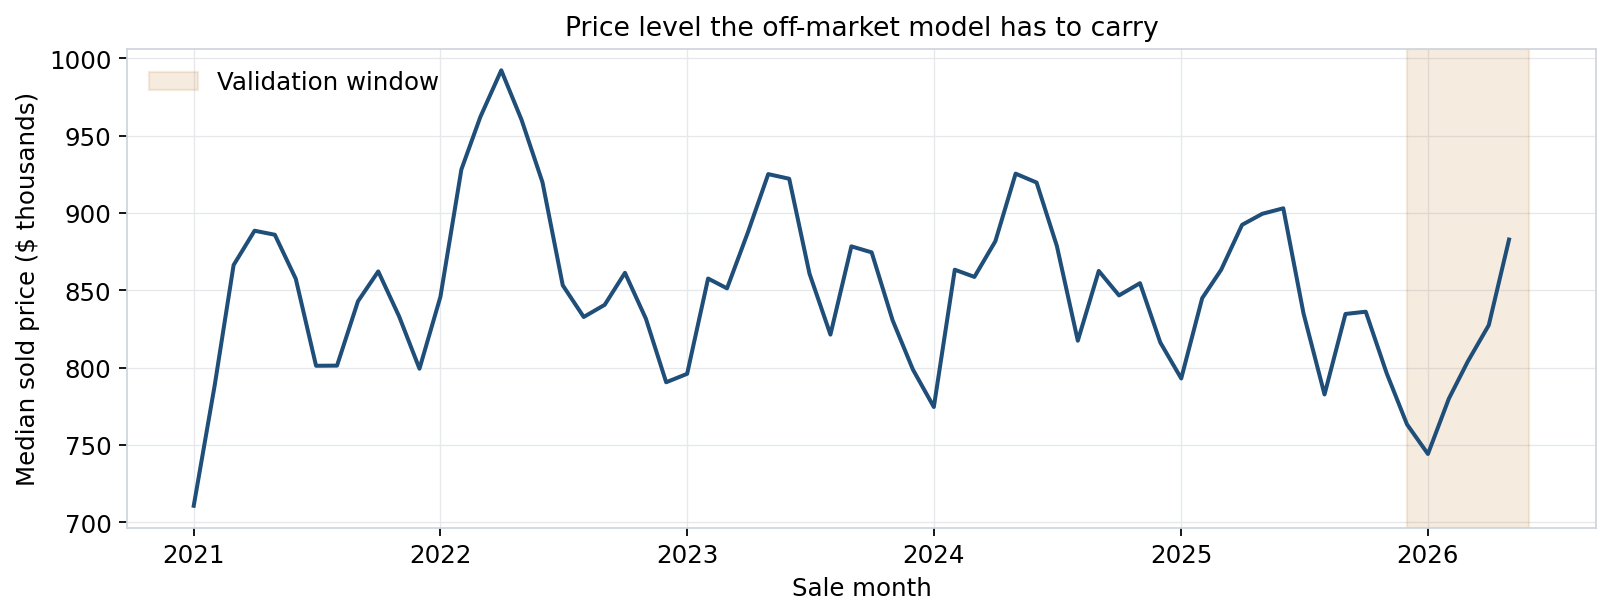
\includegraphics[width=\linewidth]{om_monthly_price.png}
\caption{Median sold price by month. The shaded band is the validation window. There is no asking price in this chart, because the off-market model is not allowed to use one.}
\label{fig:monthly}
\end{figure}

The price level is not a fixed mean. On the monthly median sold price, an augmented Dickey--Fuller test with a trend gives \(p = 0.033\), and a KPSS test with a trend does not reject stationarity around that trend (statistic \(0.093\), below the \(10\%\) critical value \(0.119\)). A robust STL split gives seasonal strength \(0.80\): May high, January low, a swing of about \(\$144{,}000\) around the trend. The seasonal pair in the feature set is there because of this swing. It is a small share of gain once community prices and building comps are present, which is consistent with those comps already carrying the recent level.

A log-linear regression on the numeric design, with no community and no comps, has \(R^2 = 0.713\) and a square-foot elasticity of \(0.496\) (standard error \(0.003\)). Residual skew is \(0.32\), against \(5.79\) for the same regression in dollars. The log scale is the one a squared-error model can live with. Developmental MdAPE of this regression is \(20.26\%\), worse than the community anchor. Attributes without a recent price do not locate a Toronto home. That is why the specification spends its complexity on comps and on a recent level correction, not on a richer linear hedonic.

\section{Feature specification}
\label{sec:features}

The tree sees 35 columns. None of them is the home's own sold price, a later sale, or the list price. The first 16 are the cleaned attributes from Section~\ref{sec:clean}, including type, style, community, and municipality as categoricals. The other 19 are variables we build. This section is the formula for each of those 19, and the reason we built it.

Category levels are the values seen in the estimation sample. A community or a style that shows up later is left missing, and LightGBM keeps the missing value. We do not map it to a nearest label.

\subsection{Community and city price levels}
\label{sec:psf}

A home with no ask still needs a local price tape. We build that tape in dollars per square foot, from sales that closed before the listing month, and we hand the tree the log.

Write \(p_j = Y_j / S_j\) for a past sale, and write \(m_j\) for its sale month as \(12\times\text{year} + \text{month}\). For a home listed in month \(\tau_i\), the community cell is the same community and the same property type. With window \(W = 12\),
\[
\mathcal{C}_i = \{ j : \text{same community and type},\ \tau_i - W \le m_j < \tau_i \}.
\]
The upper bound is strict, so a sale in the listing month is not in the cell. If \(\mathcal{C}_i\) is empty, we walk back to the latest sale of that cell before \(\tau_i\) and take a block of the same length ending at that sale. The cell median and the cell count are
\[
q^{\mathrm{comm}}_i = \operatorname{median}\{p_j : j \in \mathcal{C}_i\}, \qquad n^{\mathrm{comm}}_i = |\mathcal{C}_i|.
\]
We compute the same two numbers inside property type only, \(q^{\mathrm{type}}_i\) and \(n^{\mathrm{type}}_i\), and one citywide median \(q^{\mathrm{city}}_i\) with the same window and the same empty-window rule. The level we keep is
\[
q_i =
\begin{cases}
q^{\mathrm{comm}}_i & \text{if } n^{\mathrm{comm}}_i \ge 30,\\
q^{\mathrm{type}}_i & \text{if } n^{\mathrm{comm}}_i < 30 \text{ and } n^{\mathrm{type}}_i \ge 30,\\
q^{\mathrm{city}}_i & \text{otherwise.}
\end{cases}
\]
If that choice is still missing or not positive, we fall back to the median of \(p_j\) over every usable sale in the sample the table was built on. The column is the log,
\[
\texttt{log\_community\_psf}_i = \log q_i.
\]
On the developmental validation rows the community cell itself is the one we use for \(76\%\) of homes. The other \(24\%\) are thin cells, and they take the type or the city.

Two companions ignore the community and the type and use only the citywide median, one with a 3-month window and one with a 12-month window:
\[
\texttt{log\_city\_psf\_3}_i = \log q^{\mathrm{city},(3)}_i, \qquad
\texttt{log\_city\_psf\_12}_i = \log q^{\mathrm{city},(12)}_i.
\]
We put them in so a thin community still has a short tape and a year tape. The 3-month column moves when the market has just turned. The 12-month column is the slower level.

We picked \(W = 12\) on July--November 2025, against 6 months, 24 months, and the full history. On that slice the 12-month anchor had MdAPE \(15.33\), the 6-month \(16.19\), the 24-month \(15.70\), and the full history \(16.42\) with signed error \(+11.97\%\). Six months was noisy. The full history was stale and high. Twelve months was the lowest error, so we froze it.

In V6 we reopened the threshold of 30. The alternative was a blend that gives the community a weight \(n/(n + \text{strength})\) and gives the rest of the weight to the type median. July--November preferred the hard cut. We kept the hard cut.

\subsection{Same-pin sales}
\label{sec:building}

The community median says what homes like this sold for nearby. It does not say what this building sold for. We add that as two columns, and only from sales that closed before the home was listed.

The pin is the one in Section~\ref{sec:clean}. A comp has the same pin, a sold date strictly before \texttt{date\_listed}, and a different listing number, so a training row cannot be its own comp.

A 2022 sale and a 2025 sale of the same condo are not in the same dollars. We reindex each comp to the listing month with a type-level index that itself uses only earlier months. For property type \(t\) and month \(m\), let \(\ell_{t,m}\) be the median of \(\log p_j\) among sales of that type in that month. A month with no sale inherits the previous month's \(\ell\) (forward fill). The index we look up is then shifted back one month and smoothed over three months:
\[
I_{t,m} = \operatorname{median}(\ell_{t,m-1},\, \ell_{t,m-2},\, \ell_{t,m-3}).
\]
Month \(m\) never sees a sale from month \(m\). We store each historical sale with the market level taken out,
\[
f_j = p_j \,\exp(-I_{t(j), m(j)}).
\]
For home \(i\), write \(\mathcal{B}_i\) for the eligible comps and \(\tau_i\) for its listing month. If \(\mathcal{B}_i\) has at least one sale,
\[
\widetilde p_i = \exp(I_{t(i), \tau_i}) \times \operatorname{median}\{f_j : j \in \mathcal{B}_i\},
\]
\[
\texttt{building\_log\_price}_i = \log(S_i \,\widetilde p_i), \qquad
\texttt{building\_sales}_i = |\mathcal{B}_i|.
\]
If there is no eligible comp, the log price is missing and the count is 0. LightGBM splits on that missingness. Those homes fall back on the community level, the city level, and size.

The gate is one prior sale. On July--November, requiring three prior sales was worse, and so was adding the last sale as its own column, and so was a repeat-sale column that asked for the same beds, baths, and area string. We also tried using the building price as the base the tree predicts around, in place of the community anchor. That was worse too. The building price stays a feature. The tree decides when to trust it.

On the developmental validation rows, \(59.8\%\) of homes have at least one eligible earlier sale at the same pin.

\subsection{Phrase flags}

The remarks are free text. The cheapest use of them is a set of flags for words we already know mean something about condition or about the seller. Each flag is 1 when the pattern matches the lower-cased remarks, and 0 otherwise:
\[
\texttt{flag}_{i,k} = \mathbf{1}\{\text{pattern } k \text{ matches remarks}_i\}.
\]

\begin{center}
\small
\begin{tabular}{llp{7.2cm}}
\toprule
Flag & Pattern & Why it is here \\
\midrule
\texttt{as\_is} & as-is, as is & Condition, sold without work \\
\texttt{turnkey} & turnkey & Condition, nothing to do \\
\texttt{potential} & potential & Upside language \\
\texttt{original} & original & Unrenovated \\
\texttt{finished} & finished & A finished basement or a finished unit \\
\texttt{renovated} & renovat & Work already done \\
\texttt{needs\_work} & needs work & Work still to do \\
\texttt{stunning} & stunning, beautiful, gorgeous, spectacular & Listing praise \\
\texttt{investor} & investor, investors & Who the listing is talking to \\
\texttt{motivated} & motivated & A seller who wants out \\
\texttt{redone} & redone, redo & Work already done, said a different way \\
\texttt{dated} & dated & Condition \\
\texttt{worn} & worn & Condition \\
\bottomrule
\end{tabular}
\end{center}

The first eight were the base set. We added the last five because, on the predecessor model, the extra set cut July--November MdAPE from \(8.41\) to \(8.33\). Each flag on its own is under \(0.5\%\) of gain on the final tree. We kept the bundle because that screen, which was not allowed to see December, kept it. We would not describe the flags as drivers.

\subsection{The remarks score}

Flags only catch the phrases we wrote down. The remarks score lets the rest of the wording in, as one number, with two restrictions so it cannot cheat.

Before the vectorizer runs we rewrite the text. Any number, including a number with commas or a decimal, is replaced by the token \texttt{NUM}. Any community name of four or more characters is replaced by the token \texttt{COMMUNITY}. A printed price or a neighbourhood name then cannot be a feature of the score. We tokenize on letters only, build unigrams and bigrams, drop terms that appear in fewer than 40 documents, and keep at most 3{,}000 terms. Term frequency is sublinear, so a word repeated five times is not five times the evidence.

The score is a ridge regression of log sold price on that TF--IDF matrix, with penalty \(0.3\):
\[
r_i = \alpha_0 + \sum_{v=1}^{V} \alpha_v \,\mathrm{tfidf}_{i,v}, \qquad V \le 3000,
\]
and \(\texttt{remarks\_score}_i = r_i\). It is in log-price units. It is a feature, not a prediction we average with the tree.

Inside the estimation sample a row cannot help fit the ridge that scores it. We sort the sample by sold date and cut it at \(40\%\), \(55\%\), \(70\%\), \(85\%\), and \(100\%\) of the rows. The block from \(40\%\) to \(55\%\) is scored by a ridge fit on the first \(40\%\). The next block is scored by a ridge fit on everything before it, and so on. The first \(40\%\) of rows have no score, and the tree sees those as missing. A home we are scoring, which is not in the fit sample, gets the ridge fit on the whole past. Its own sale is not in that past.

July--November preferred the score. Inner MdAPE was \(7.97\) with it and \(8.02\) without it, both with the level shift on. The margin is \(0.05\) points, and the gain share on the developmental tree is \(0.7\%\). We kept it because the screen kept it. The comps are doing the work.

\subsection{The 35 columns, in one place}

\begin{center}
\small
\begin{tabular}{llp{6.6cm}}
\toprule
Column & Count & Where it comes from \\
\midrule
Size, lot, counts, lat, lon & 10 & Section~\ref{sec:clean}. \(\log S\), the lot treatment, four counts, two coordinates. \\
Listing-month pair & 2 & \(\sin(2\pi m/12)\) and \(\cos(2\pi m/12)\). \\
\texttt{log\_community\_psf} & 1 & \(\log q_i\), the 12-month fallback above. \\
City tapes & 2 & \(\log q^{\mathrm{city}}\) over 3 months and over 12. \\
Type, style, community, municipality & 4 & Categorical. Levels frozen on the estimation sample. \\
Phrase flags & 13 & The table above. \\
\texttt{building\_sales}, \texttt{building\_log\_price} & 2 & Prior same-pin count, and \(\log(S\widetilde p)\). \\
\texttt{remarks\_score} & 1 & Time-safe ridge on the cleaned remarks. \\
\midrule
Total & 35 & \\
\bottomrule
\end{tabular}
\end{center}

\subsection{What the splits actually use}
\label{sec:gain}

\begin{figure}[ht]
\centering
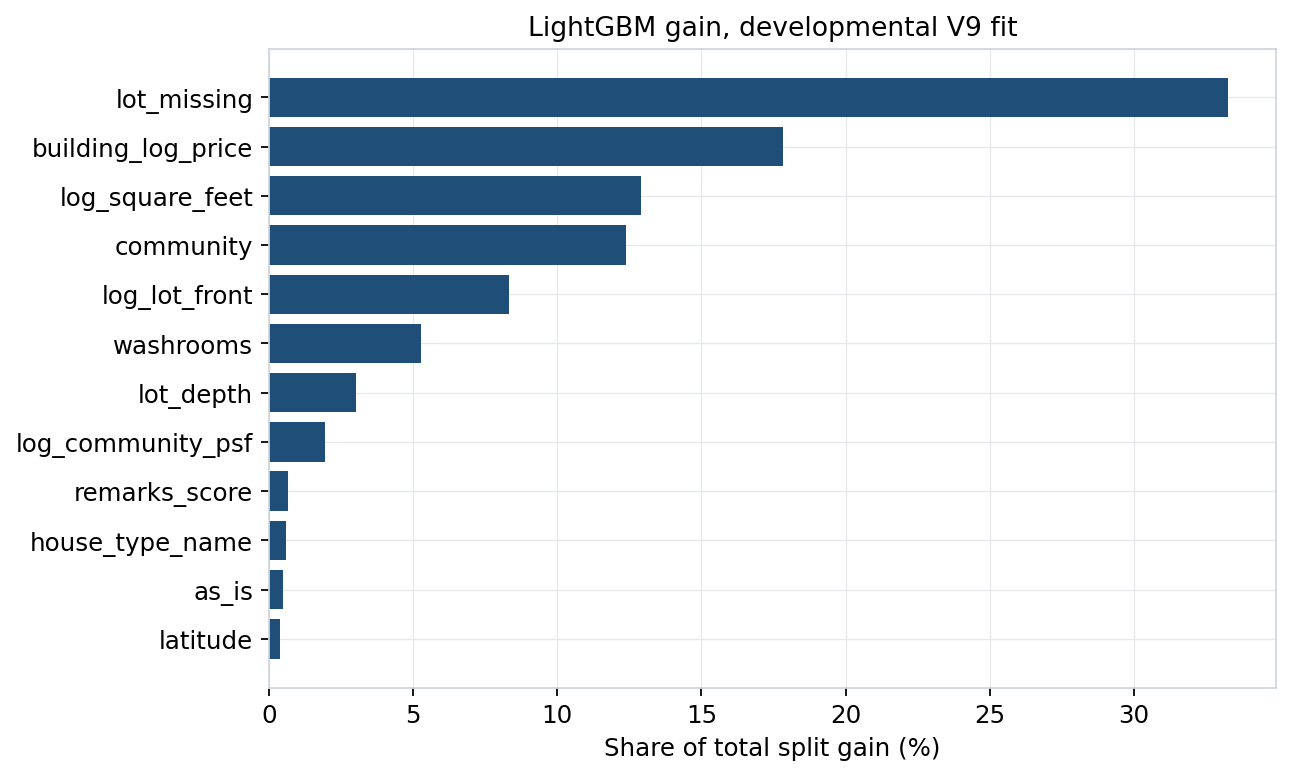
\includegraphics[width=0.92\linewidth]{om_feature_gain.png}
\caption{Share of total LightGBM split gain on the developmental \modelid{} fit. Gain describes the fitted tree. It is not a causal ranking.}
\label{fig:gain}
\end{figure}

\begin{center}
\begin{tabular}{lr l}
\toprule
Feature & Gain share & Reading \\
\midrule
\texttt{lot\_missing} & 33.3\% & The house-versus-apartment cut \\
\texttt{building\_log\_price} & 17.8\% & Reindexed same-pin price, when a comp exists \\
\texttt{log\_square\_feet} & 12.9\% & Size \\
\texttt{community} & 12.4\% & Neighbourhood level \\
\texttt{log\_lot\_front} & 8.3\% & Frontage, on homes that have a lot \\
\texttt{washrooms} & 5.3\% & The count with the largest linear coefficient \\
\texttt{lot\_depth} & 3.0\% & Lot, on houses \\
\texttt{log\_community\_psf} & 2.0\% & The 12-month local tape \\
\texttt{remarks\_score} & 0.7\% & Small once comps are in the tree \\
\bottomrule
\end{tabular}
\end{center}

Municipality is \(0\%\) of gain once community is present. Individual phrase flags are each under \(0.5\%\). We selected them as a bundle on an earlier model, and we did not rerun an isolated deletion on the final specification, so they stay. We would not describe them as drivers.

\subsection{Decisions that were tested and not kept}

\begin{center}
\small
\begin{tabular}{p{4.4cm}p{9.0cm}}
\toprule
Candidate & What happened \\
\midrule
Predict the gap around the community anchor (V3--V8) & Walk-forward MdAPE \(7.50\%\) for the best of these, against \(7.45\%\) for the direct model. \\
Blend the community median with the type median & July--November preferred the hard threshold of 30 sales. \\
Three prior sales, last sale, repeat sale & Worse than one prior sale on July--November. \\
Separate house and condo shifts & July--November MdAPE \(8.18\) against \(8.17\) for one shift, on the gap model. \\
A 75/25 blend of the direct model and the gap model & Tied the pure direct model on July--November. The pure model was kept. \\
Quantile loss at the median & Walk-forward MdAPE \(7.53\%\), behind the squared-error direct model. \\
A land-value term and a drifting city forecast (V8) & July--November preferred no land term and a flat forecast, which collapsed V8 back to V7. \\
\bottomrule
\end{tabular}
\end{center}

\section{Estimation and calibration}
\label{sec:calibration}

The tree predicts log sold price. It has no intercept we can edit by hand, and on a market that has just moved it comes out a little high or a little low for every home at once. Calibration is the step where we measure that common miss on a recent slice the tree has not seen, and we scale every prediction by the same factor.

\subsection{The fitted equation}

Let \(x_i\) be the 35-column design. The tree gives a raw price
\[
\log \tilde Y_i = F_{\hat\theta}(x_i), \qquad \tilde Y_i = \exp\bigl(F_{\hat\theta}(x_i)\bigr).
\]
The number we report is
\[
\hat Y_i = \tilde Y_i \,\exp(-w\,\delta),
\]
where \(\delta\) is one number for the whole book and \(w\) is a weight we choose before we open December. With \(w = 1\), which is what we shipped, this is a single percent applied to every home. With \(w = 0\) the raw tree is the prediction.

\(\delta\) is a median log error, not a mean. On the three months before the origin, using a tree that was fit only before those three months,
\[
\delta = \operatorname{median}\bigl(\log \tilde Y_j - \log Y_j\bigr).
\]
A positive \(\delta\) means the raw tree is high, and \(\exp(-\delta)\) pulls every prediction down. We use the median so one \(\$30\) million miss does not set the factor.

\subsection{How we measure the shift on the developmental split}

The origin is 30 November 2025. We run two fits, because the months that teach us the bias cannot also be inside the tree that we are judging.

\begin{enumerate}
\item Fit the price tables, the building comps, the remarks ridge, and the tree on sales closed before 1 September 2025.
\item Score September, October, and November 2025 with that tree. Those three months are in none of the tables and in none of the trees.
\item Set \(\delta\) to the median of \(\log\tilde Y - \log Y\) on those three months.
\item Refit the tables, the comps, the ridge, and the tree on every sale through 30 November 2025.
\item Score December 2025 through May 2026 with the refit tree, and multiply by \(\exp(-\delta)\).
\end{enumerate}

The September--November miss was \(\delta = +0.0158\) in log price, which is \(+1.58\%\) as a price factor because \(\exp(\delta) - 1 = 0.0159\). The raw tree was high. The correction multiplies every December--May prediction by \(\exp(-0.0158) \approx 0.984\).

Walk-forward does the same two-fit procedure one month at a time. For a sale month \(m\), \(\delta\) is the median log miss on the three months before \(m\), from a tree fit only before those three months, and the scoring tree is fit on everything before \(m\). We do not reuse the September--November number in January.

\subsection{Settings we froze}

We did not run a new grid once the comps were in the design. We reused the settings already selected for the list-aware model, because they had already travelled and because LightGBM takes the community and the type as native categories.

\begin{center}
\begin{tabular}{ll}
\toprule
Setting & Value \\
\midrule
Objective & Squared error on \(\log Y\) \\
Trees & 700 \\
Leaves per tree & 127 \\
Learning rate & 0.03 \\
Minimum rows in a leaf & 20 \\
Row subsample & 0.8, every tree \\
Column subsample & 0.8 \\
L2 penalty on leaf weights & 1 \\
Seed & 0 \\
\bottomrule
\end{tabular}
\end{center}

Earlier, on the attribute block alone, a small grid picked an XGBoost of depth 10, learning rate \(0.05\), and 600 trees. Its developmental MdAPE was \(17.28\%\), behind the community anchor. CatBoost on that block was \(18.61\%\) and a random forest \(18.95\%\). Once we had categoricals and comps we moved the engine to LightGBM and kept the settings above. Another booster could match this. We did not spend the search there. The error was moving when we changed the columns, not when we changed the depth.

\subsection{How we chose the weight}

The screen is July--November 2025, and it is not allowed to see December. Inside the screen the dates are pulled forward so that July is scored by a model that has not seen July:

\begin{center}
\small
\begin{tabular}{ll}
\toprule
Piece & Sales we allow it to see \\
\midrule
Tree that measures \(\delta\) & Closed before 1 April 2025 \\
Months \(\delta\) is measured on & April, May, June 2025 \\
Tree that scores the slice & Closed before 1 July 2025 \\
Slice we judge & July through November 2025 \\
\bottomrule
\end{tabular}
\end{center}

On that slice, for the direct model with the remarks score, we tried the two ends of the weight.

\begin{center}
\begin{tabular}{lrr}
\toprule
Weight & MdAPE & Median signed error \\
\midrule
\(w = 0\), raw tree & 8.31 & \(+4.71\%\) \\
\(w = 1\), full shift & 7.97 & \(+3.77\%\) \\
\bottomrule
\end{tabular}
\end{center}

Full weight was better on the absolute error and on the bias, so we set \(w = 1\). The slice is still \(+3.77\%\) high after the shift. That leftover is why a later month gets its own \(\delta\). A factor estimated on April--June is the right size for July--November only in part. December gets a factor estimated on September--November, and each walk-forward month gets a factor estimated on the three months just before it.

We also tried letting the factor differ by broad type. Detached, semi-detached, and freehold townhouse share one median log miss, and the other types share another:
\[
\hat Y_i =
\begin{cases}
\tilde Y_i \exp(-\delta_{\mathrm{house}}) & \text{if the type is a house},\\
\tilde Y_i \exp(-\delta_{\mathrm{condo}}) & \text{otherwise}.
\end{cases}
\]
On the gap model, which is where we ran this comparison, July--November MdAPE was \(8.18\) with the two factors and \(8.17\) with one factor. We kept one factor. A decile-specific factor was not part of the search. The plot below is why we would be careful with one anyway.

\subsection{What the calibration plot shows}

\begin{figure}[ht]
\centering
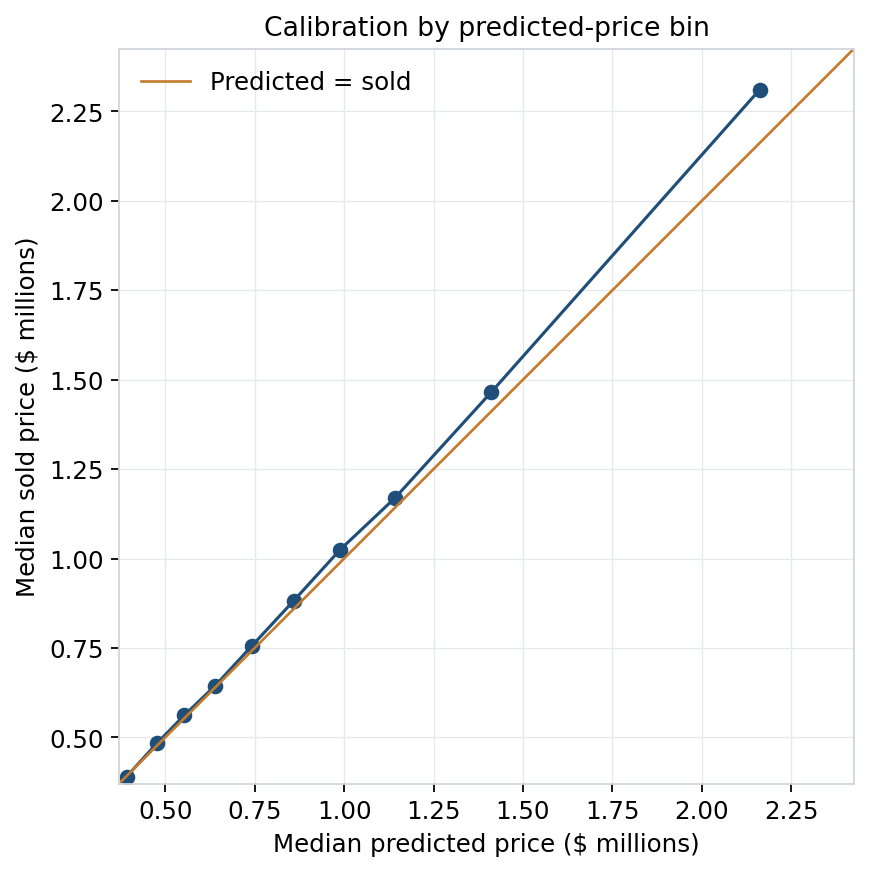
\includegraphics[width=0.64\linewidth]{om_calibration.png}
\caption{Developmental validation, after the \(+1.58\%\) shift. Homes are grouped into ten bins of predicted price. Each point is the median prediction against the median sold price.}
\label{fig:cal}
\end{figure}

We bin the validation sales by the predicted price and plot the median prediction in the bin against the median sold price. The bins rise together from under \(\$0.5\) million to a little above \(\$2\) million. Through the middle of the book the medians sit on the diagonal, so the ordering is right and the level is about right. The top bin falls off the line: the median home in that predicted-price bin sold for more than the bin's median prediction. Section~\ref{sec:errors} shows the same fact from the other direction. Slicing by sold price, the cheapest decile has median signed error \(+2.5\%\) and the top decile has \(-10.7\%\).

One percent applied to every home moves the cheap end and the expensive end by the same amount. Pulling the top decile up would push the bottom decile, which is already a bit high, further high. That is the limit of this calibration. It corrects a common level. It does not correct a bias that changes sign across the price range. We left it as one number because the two-type version did not earn its place on the pre-December screen, and because a richer correction fit on the validation months would be using the months we are supposed to be scoring.

\FloatBarrier
\section{Architecture}
\label{sec:architecture}

\modelid{} is one tree on log price, with three upstream constructions and one level correction. The upstream pieces do not produce a price that is then averaged. They produce columns. The correction is the only second stage, and it is a single percent.

\begin{figure}[ht]
\centering
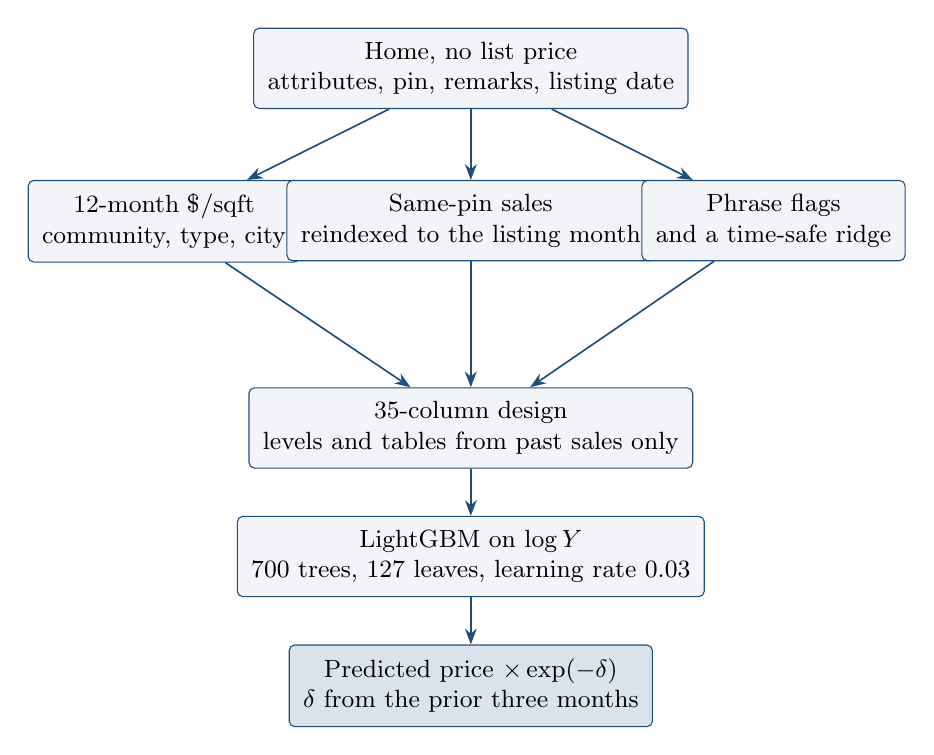
\begin{tikzpicture}[
  font=\small,
  box/.style={draw=navy, rounded corners=2pt, align=center, inner sep=5pt,
              minimum height=8mm, fill=navy!6},
  arr/.style={-{Stealth[length=2mm]}, semithick, draw=navy}
]
\node[box] (raw) {Home, no list price\\ attributes, pin, remarks, listing date};
\node[box, below left=9mm and -6mm of raw] (psf) {12-month \$/sqft\\ community, type, city};
\node[box, below=9mm of raw] (pin) {Same-pin sales\\ reindexed to the listing month};
\node[box, below right=9mm and -6mm of raw] (text) {Phrase flags\\ and a time-safe ridge};
\node[box, below=16mm of pin] (design) {35-column design\\ levels and tables from past sales only};
\node[box, below=6mm of design] (lgb) {LightGBM on \(\log Y\)\\ 700 trees, 127 leaves, learning rate 0.03};
\node[box, below=6mm of lgb, fill=navy!16] (out) {Predicted price \(\times \exp(-\delta)\)\\ \(\delta\) from the prior three months};
\draw[arr] (raw) -- (psf);
\draw[arr] (raw) -- (pin);
\draw[arr] (raw) -- (text);
\draw[arr] (psf) -- (design);
\draw[arr] (pin) -- (design);
\draw[arr] (text) -- (design);
\draw[arr] (design) -- (lgb);
\draw[arr] (lgb) -- (out);
\end{tikzpicture}
\caption{Scoring path for \modelid{}. A building comp must have closed before the listing date. \(\delta\) is fit without the months it is measured on, and without the month being scored.}
\label{fig:flow}
\end{figure}

The rejected alternative is the gap model. It prices the home as the community anchor times a tree. That path is V3 through V7. It is a good model, half a point of walk-forward MdAPE behind this one, and it remains the challenger in Section~\ref{sec:challengers}. V8 tried to add a land component and a drifting forecast of the city level. The pre-December screen turned both off, so V8's scored predictions are V7's predictions.

\FloatBarrier
\section{Developmental evidence}
\label{sec:develop}

One origin, 30 November 2025. Fit on 139{,}931 sales. Score 10{,}069 sales.

\begin{center}
\begin{tabular}{lrrr}
\toprule
Model & MdAPE & MAPE & Median signed \\
\midrule
OLS, raw dollars & 21.76 & 29.54 & \(+14.16\) \\
OLS, log price & 20.26 & 27.14 & \(+11.88\) \\
All-history community \$/sqft & 17.07 & 22.23 & \(+10.84\) \\
V1, 12-month community \$/sqft & 15.60 & 20.80 & \(+3.71\) \\
V3, LightGBM on the V1 gap & 9.40 & 12.13 & \(+1.03\) \\
V7, gap plus one same-pin sale & 7.54 & 9.95 & \(-1.72\) \\
\modelid{}, direct log price & 7.53 & 9.77 & \(-2.10\) \\
\bottomrule
\end{tabular}
\end{center}

The reproduced fit adds the tail: the 90th percentile of absolute percentage error is \(20.5\%\) and the 95th is \(26.5\%\). The 12-month anchor on the same homes is \(43.4\%\) and \(56.6\%\). The model cuts the typical error in half relative to the anchor and shortens the bad tail. It does not make a \(20\%\) miss unusual.

On this one cut, \modelid{} and V7 are a hundredth of a point apart, and \modelid{} is the more biased of the two (\(-2.10\%\) against \(-1.72\%\)). The adoption does not rest on that hundredth. It rests on the July--November screen, where the direct model beat the gap model before December was opened, and on the walk-forward, where the direct model also leads and the bias shrinks.

\section{Walk-forward validation}
\label{sec:walk}

\subsection{Definition}

For each sale month \(m\) from December 2025 through May 2026:

\begin{enumerate}
\item The past is every sale with \texttt{date\_sold} strictly before the first day of \(m\).
\item Community and city tables, building comps, the remarks ridge, category levels, and the tree are rebuilt on that past.
\item \(\delta\) is the median log miss on the three months before \(m\), from a tree fit only before those three months.
\item Month \(m\) is scored. Its sold prices are not in any table and not in the tree.
\item The six months are concatenated. Pooled MdAPE weights homes equally. May, with \(2{,}291\) sales, weighs more than January, with \(1{,}058\).
\end{enumerate}

A building comp inside that refit still has to predate the home's listing. The July--November choices, including shift weight 1 and the remarks score, stay fixed. They are not re-searched inside the walk.

The month-by-month V9 numbers below are the stored outputs of the notebook. The reproduction script refit the developmental model and matched it. It did not repeat the six walk-forward refits. A random \(k\)-fold split is not a substitute. It leaks later sales into the community medians and the building comps.

\subsection{Results}

\begin{figure}[ht]
\centering
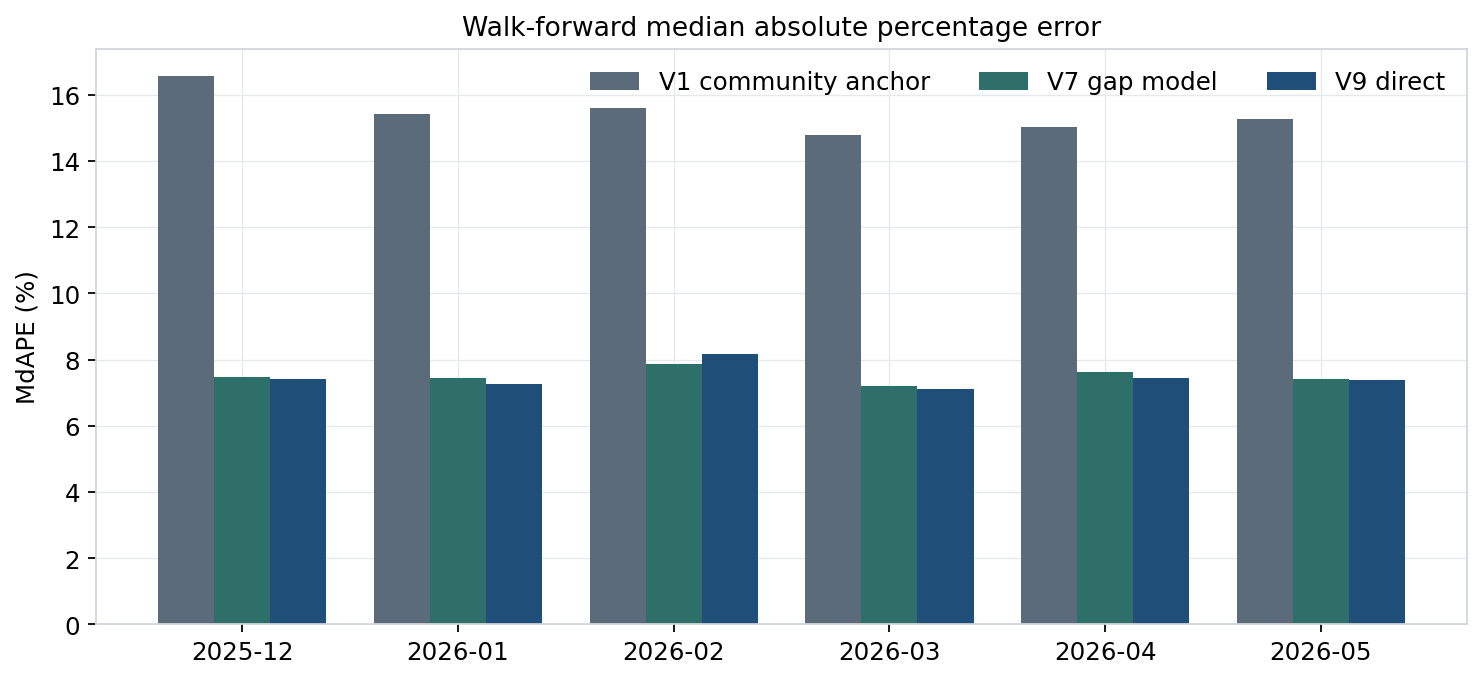
\includegraphics[width=\linewidth]{om_walkforward_mdape.png}
\caption{Walk-forward MdAPE by sale month. V1 is the 12-month community anchor. V7 is the best gap model. V9 is \modelid{}.}
\label{fig:wf}
\end{figure}

\begin{center}
\small
\begin{tabular}{l r rrr rr}
\toprule
 & & \multicolumn{3}{c}{MdAPE} & \multicolumn{2}{c}{V9 signed} \\
\cmidrule(lr){3-5} \cmidrule(lr){6-7}
Month & Homes & V1 & V7 & V9 & V7 & V9 \\
\midrule
2025-12 & 1{,}238 & 16.57 & 7.49 & 7.42 & \(+0.97\) & \(+0.63\) \\
2026-01 & 1{,}058 & 15.43 & 7.44 & 7.27 & \(-2.93\) & \(-2.50\) \\
2026-02 & 1{,}442 & 15.61 & 7.86 & 8.17 & \(-3.79\) & \(-4.44\) \\
2026-03 & 1{,}816 & 14.79 & 7.19 & 7.10 & \(-1.03\) & \(-1.15\) \\
2026-04 & 2{,}224 & 15.02 & 7.64 & 7.44 & \(+1.72\) & \(+1.65\) \\
2026-05 & 2{,}291 & 15.28 & 7.40 & 7.39 & \(-0.05\) & \(+0.98\) \\
\midrule
Pooled & 10{,}069 & 15.33 & 7.50 & 7.45 & \(-0.50\) & \(-0.37\) \\
\bottomrule
\end{tabular}
\end{center}

Pooled MAPE is \(20.32\%\) for V1, \(9.91\%\) for V7, and \(9.79\%\) for V9.

\begin{figure}[ht]
\centering
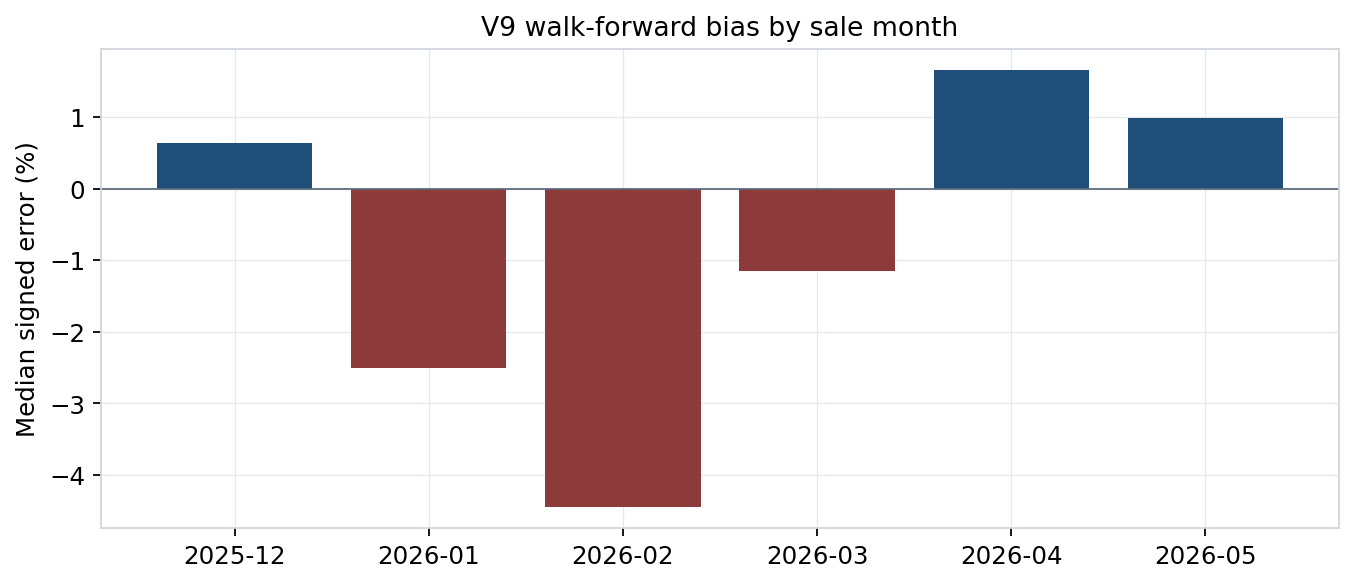
\includegraphics[width=0.92\linewidth]{om_walkforward_bias.png}
\caption{Walk-forward median signed percentage error of \modelid{}. The pool is near zero. February is not.}
\label{fig:bias}
\end{figure}

\subsection{What this comparison decides}

V9 beats V7 in five of the six months. February is the exception: V9 MdAPE \(8.17\) against V7 \(7.86\), and V9 is \(4.44\%\) low. The pooled margin is \(0.05\) points. That is a small lead, in the same direction as the pre-December screen, and it is not a month-by-month domination. The direct model is adopted because it won the screen it was allowed to win and then did not lose the out-of-time test. It is not adopted because \(7.45\) against \(7.50\) is a large economic gap. V7 stays the challenger.

The pooled bias of \(-0.37\%\) is not a license to call the model unbiased. The monthly signed error runs from \(-4.44\%\) to \(+1.65\%\). February is a level miss the three-month correction did not catch in time. A user who marks one month to this model can be several percent off even when the half-year pool looks calm.

\subsection{A stale book}
\label{sec:stale}

The notebook scores May 2026 a second time with sales cut off at the end of January, which is the situation if the comps are about three months old. For the direct model, May's MdAPE moves from \(7.39\%\) to \(8.38\%\), and the median signed error moves from \(+0.98\%\) to \(-5.29\%\). The same cut on the median-loss variant moves May from \(7.45\%\) to \(8.83\%\). A delayed tape makes the model cheap. The off-market test file lists homes from August 2025 through September 2026, so the age of the last sale in the tables is part of the operating design, not a footnote.

\subsection{Challengers under the same protocol}
\label{sec:challengers}

\begin{center}
\begin{tabular}{lrrr}
\toprule
Model & MdAPE & MAPE & Median signed \\
\midrule
V1, 12-month community \$/sqft & 15.33 & 20.32 & \(+3.19\) \\
V2, V1 plus a level shift & 14.96 & 19.11 & \(-2.42\) \\
V4, gap model plus a level shift & 9.04 & 11.70 & \(-1.11\) \\
V5, V4 plus base phrases & 8.64 & 10.89 & \(-1.29\) \\
V6, extra phrases, full shift & 8.56 & 10.88 & \(-1.23\) \\
V7, one same-pin sale & 7.50 & 9.91 & \(-0.50\) \\
V9 median loss on the V7 gap & 7.53 & 10.05 & \(-0.64\) \\
\modelid{} & 7.45 & 9.79 & \(-0.37\) \\
\bottomrule
\end{tabular}
\end{center}

V8 is absent because its selected specification was V7. The land term and the drifting forecast did not survive July--November, and the walk-forward path of V8 matches V7 sale for sale.

The median-loss tree beats the direct model in December (\(7.23\) against \(7.42\)) and in February (\(7.99\) against \(8.17\)). It loses the other four months and the pool. Matching the training loss to MdAPE more literally did not produce a better out-of-time median.

\section{Error analysis}
\label{sec:errors}

Segmented errors are from the developmental refit (one origin, MdAPE \(7.53\%\)). They are not a second walk-forward. The developmental signed error is \(-2.10\%\), more negative than the walk-forward pool, because one shift estimated on September--November was applied to the whole half year.

\begin{figure}[ht]
\centering
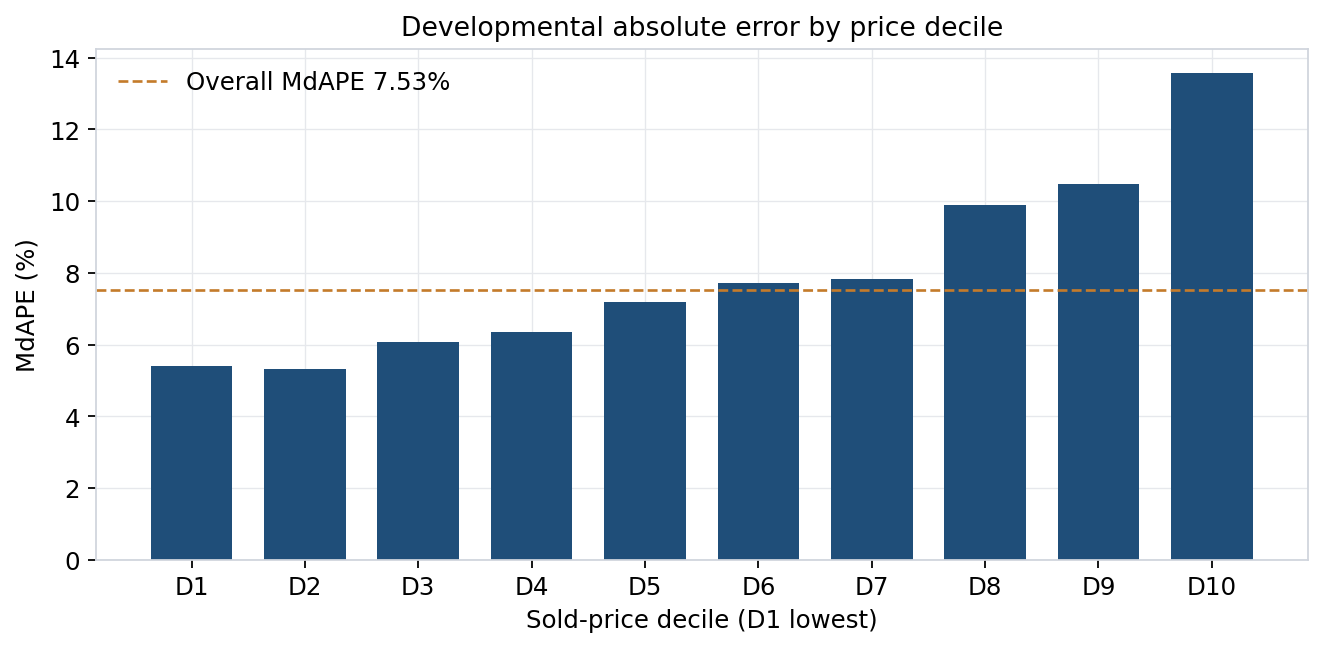
\includegraphics[width=0.92\linewidth]{om_error_by_decile.png}
\caption{Developmental MdAPE by sold-price decile. The dashed line is the overall \(7.53\%\).}
\label{fig:decile}
\end{figure}

\begin{center}
\small
\begin{tabular}{lrrrrr}
\toprule
Decile & Homes & Sold price, from & Sold price, to & MdAPE & Median signed \\
\midrule
D1 & 1{,}007 & 226{,}200 & 440{,}400 & 5.40 & \(+2.53\) \\
D2 & 1{,}008 & 440{,}500 & 521{,}000 & 5.33 & \(-0.50\) \\
D3 & 1{,}006 & 521{,}100 & 597{,}000 & 6.07 & \(-0.78\) \\
D4 & 1{,}007 & 597{,}100 & 692{,}000 & 6.36 & \(-1.31\) \\
D5 & 1{,}009 & 692{,}100 & 805{,}300 & 7.19 & \(-0.08\) \\
D6 & 1{,}004 & 805{,}400 & 939{,}200 & 7.71 & \(-1.63\) \\
D7 & 1{,}007 & 939{,}300 & 1{,}101{,}000 & 7.84 & \(-2.76\) \\
D8 & 1{,}007 & 1{,}101{,}100 & 1{,}316{,}300 & 9.88 & \(-5.63\) \\
D9 & 1{,}007 & 1{,}316{,}800 & 1{,}761{,}200 & 10.47 & \(-6.71\) \\
D10 & 1{,}007 & 1{,}761{,}400 & 17{,}035{,}700 & 13.58 & \(-10.68\) \\
\bottomrule
\end{tabular}
\end{center}

Error rises with price. The bottom half of the book, under about \(\$800{,}000\), is where the model is sharpest. The top decile is a different product: MdAPE \(13.6\%\), and the predictions are about \(11\%\) low. The cheapest decile is biased the other way, \(+2.5\%\). A user marking luxury collateral to this model will be systematically cheap. A user marking the bottom of the book will be slightly rich. This is the opposite shape from LA-V22, which was tightest in the middle and high on the cheapest decile. The two models fail in different places.

\begin{figure}[ht]
\centering
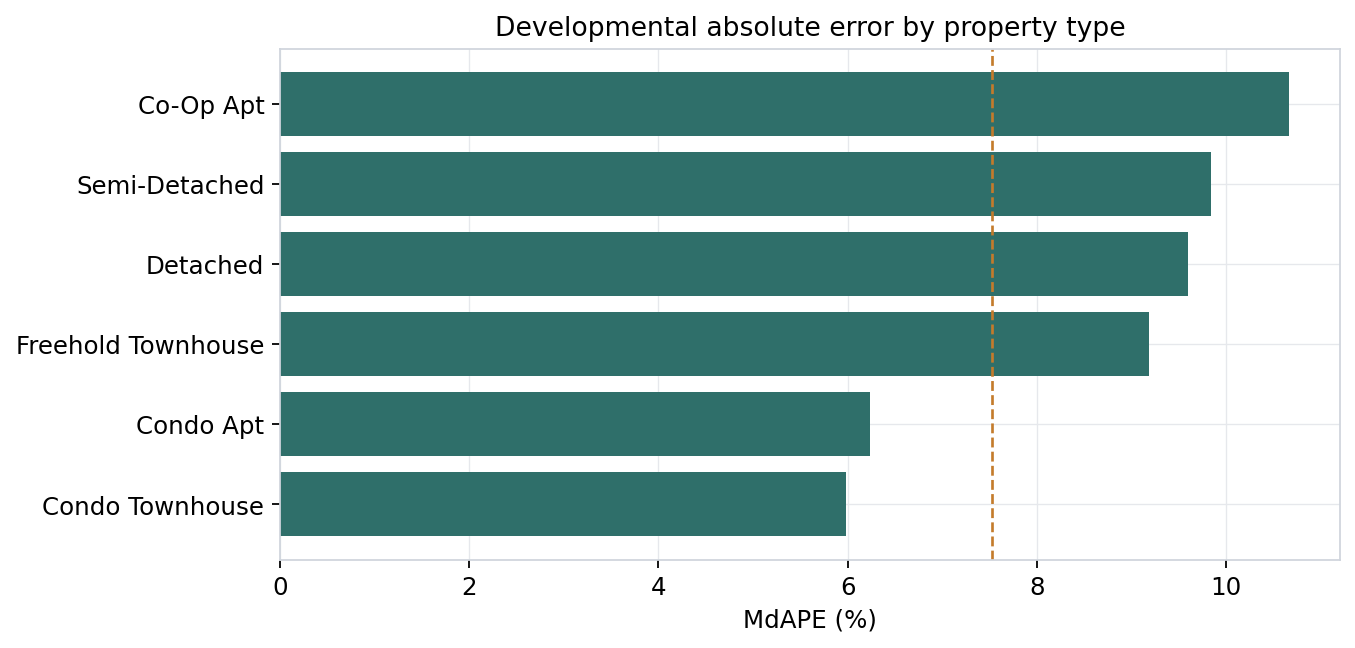
\includegraphics[width=0.88\linewidth]{om_error_by_type.png}
\caption{Developmental MdAPE by property type. The dashed line is the overall \(7.53\%\).}
\label{fig:type}
\end{figure}

\begin{center}
\begin{tabular}{lrrrr}
\toprule
Type & Homes & MdAPE & MAPE & Median signed \\
\midrule
Condo townhouse & 616 & 5.98 & 7.54 & \(-1.42\) \\
Condo apartment & 4{,}843 & 6.24 & 8.09 & \(-1.54\) \\
Freehold townhouse & 405 & 9.19 & 10.97 & \(-5.14\) \\
Detached & 3{,}123 & 9.60 & 11.98 & \(-2.33\) \\
Semi-detached & 1{,}034 & 9.84 & 11.51 & \(-4.34\) \\
Co-op apartment & 48 & 10.67 & 16.75 & \(-1.47\) \\
\bottomrule
\end{tabular}
\end{center}

Apartments and condo townhouses carry the headline. Ground-oriented homes cost about three to four extra points of MdAPE, and freehold and semi-detached are several percent cheap. Co-op results rest on 48 sales. The same-pin feature is available for \(60\%\) of validation homes, and that coverage is higher where many sales share a coordinate, which is the condo stock. Houses more often have an empty pin and have to be priced from the community tape and the lot. That is a credible reason the house error is wider. It is also why \texttt{lot\_missing} dominates the gain chart: the tree's first job is to tell those two books apart.

Municipalities do not separate. Developmental MdAPE runs from \(6.32\%\) in York (\(n = 124\)) to \(7.68\%\) in Toronto (\(n = 5{,}746\)). The failure mode is price and structure.

\begin{figure}[ht]
\centering
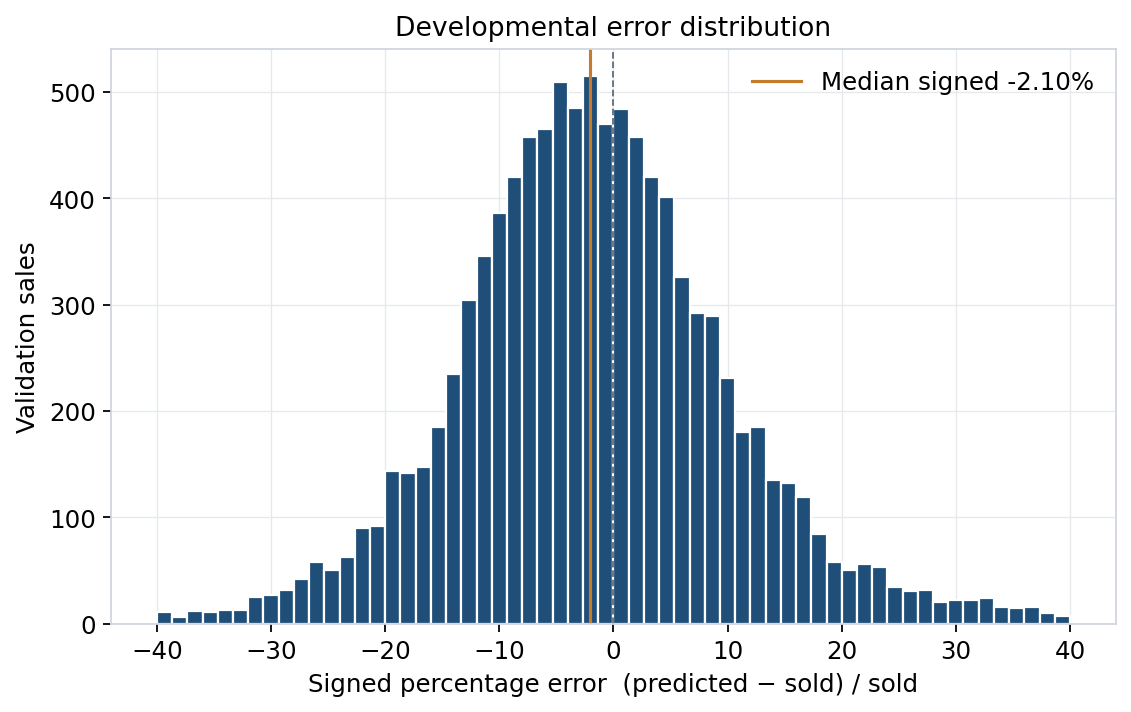
\includegraphics[width=0.86\linewidth]{om_error_distribution.png}
\caption{Developmental signed percentage error, truncated to \(-40\%\) to \(+40\%\) for display. The amber line is the median.}
\label{fig:err}
\end{figure}

MAPE (\(9.77\%\)) exceeds MdAPE (\(7.53\%\)) because of the right tail of absolute errors. A statement that the model is ``within \(10\%\)'' is false for a large minority of sales. The supported statement is: the median absolute miss is about \(7.5\%\) walked forward, the mean absolute miss is about \(9.8\%\), and about one sale in ten on the developmental window is off by more than \(20\%\).

\section{Assumptions, limitations, and model risk}
\label{sec:limits}

\begin{enumerate}
\item The book is synthetic. Coordinates must not be joined to external maps. A method that works here is evidence about this generating process.

\item The performance claim stops in May 2026. The deployment file lists homes through September 2026 and has no labels here.

\item The output is a point estimate. The 95th percentile of \(26\%\) is a description of one window, not a band that updates with the home.

\item Pooled walk-forward bias is \(-0.37\%\). Monthly bias is not. February is \(4.4\%\) low. The expensive decile of the one-shot fit is about \(11\%\) low. Users who need a mark on a single month, or on the top of the book, should not treat the pool as their error.

\item The level correction is one percent. It was selected because it helped a pre-December slice. It cannot repair a bias that changes sign across the price range.

\item Same-pin comps exist for \(60\%\) of the developmental validation homes. The rest are priced without a building sale. A new subdivision, or a house with no earlier sale at that coordinate, is in the worse half of this design.

\item Comps that are three months stale cost about one point of MdAPE on May 2026 and push the median about \(5\%\) low. The age of the sales tape is a model input in practice.

\item The remarks score won its screen by \(0.05\) points and has \(0.7\%\) of split gain. It is not the source of the model's accuracy. Phrase flags are smaller still.

\item List price, days on market, and the third-party AVM are excluded. Including the ask would answer a different question. Including the others would leak.

\item The runnable implementation is \texttt{OffMarketModel}, called from \texttt{run.py} (Section~\ref{sec:repro}). A sign-off on this document covers that entry point together with the specification and the evidence. It does not cover a separate production service. The ten-nearest-sales baseline remains in \texttt{models.py} and is not called.

\item No bootstrap interval is reported. Stability is the month path: MdAPE inside \(7.10\%\) to \(8.17\%\), bias not inside a tight band.
\end{enumerate}

\section{Ongoing monitoring}
\label{sec:monitor}

Proposed review triggers. They were not optimised as a trading rule. They sit outside the path this window actually produced.

\begin{center}
\begin{tabular}{p{5.2cm}p{8.2cm}}
\toprule
Measure & Review if \\
\midrule
Monthly MdAPE & Above \(10\%\). The observed path is \(7.1\)--\(8.2\). \\
Monthly median signed error & Outside \(\pm 5\%\). February already reached \(-4.4\%\). \\
Top decile & Median signed error below \(-12\%\) on sales over \(\$1.5\) million. \\
Same-pin coverage & Eligible earlier sale for under \(40\%\) of new homes. \\
Tape age & Last sale in the tables more than 90 days before the scoring date. The May stale test is the evidence. \\
Population & Condo share moves by more than 10 percentage points relative to the estimation book. \\
\bottomrule
\end{tabular}
\end{center}

Each score should be stored with the listing identifier, the predicted price, the model version, the month the tables were built through, and whether a same-pin comp was found. V7 should be scored beside \modelid{}. If a rolling six-month MdAPE stops favouring the direct model, the gap specification is the fallback, not the raw community anchor. The anchor remains the fail-safe quote when the tree cannot be run.

\section{Reproducibility}
\label{sec:repro}

We now have two ways to rebuild \modelid{}, and they agree on the claim. The figures and the one-origin developmental fit come from the figure script. The walk-forward, including the month path in Section~\ref{sec:walk}, is what the submission code writes. That code is the model we hand in.

\subsection{Where the submission lives}

\begin{center}
\small
\begin{tabular}{p{3.5cm}p{11.2cm}}
\toprule
File & What it does for \modelid{} \\
\midrule
\texttt{data.py} & Loads \texttt{listings} and \texttt{test\_off\_market} from Hugging Face (\texttt{Baliyang/SSU\_data\_dash}), or from the folder in \texttt{DATA\_DIR}. \texttt{hide\_answers} drops sold price, sale date, days on market, the third-party AVM, and list price before an off-market row is scored. \\
\texttt{features.py} & Columns we can read off the home: \texttt{home\_numbers} without list price, and \texttt{remark\_flags} for the thirteen phrases. \\
\texttt{models.py} & \texttt{OffMarketModel}. \texttt{fit} builds the 12-month price tables, the same-pin comps, and the remarks ridge from the sales it was given, measures \(\delta\) on the last three months of that sample, then fits LightGBM on \(\log Y\). \texttt{predict} multiplies by \(\exp(-\delta)\). \\
\texttt{run.py} & The four commands below. \texttt{make\_model("off\_market")} is the constructor it calls. \\
\texttt{check\_submission.py} & Checks the written file: one row per test id, and a positive finite price. \\
\bottomrule
\end{tabular}
\end{center}

\texttt{NearestSalesBaseline} and the starter \texttt{FeatureModel} are still in \texttt{models.py}. \texttt{run.py} does not call them. The price levels, the building comps, and the remarks score are built inside \texttt{fit}, from the training sales only. List price never enters the design. Category levels are the values seen in that training slice.

The shift window moves with the sample. \texttt{fit} takes the last sale month in the data it was given and measures \(\delta\) on that month and the two before it, using a tree fit only before those three months. The scoring tree is then fit on the whole sample, including those three months, and every prediction is multiplied by \(\exp(-\delta)\) with weight \(1\). On a sample that stops at 30 November 2025 the window is September--November, and the shift we measured is \(+1.58\%\). A later sample gets a later window. That is the same rule as the walk-forward in Section~\ref{sec:calibration}.

The tree settings are the ones in Section~\ref{sec:calibration}: 127 leaves, learning rate \(0.03\), 700 trees, seed \(0\). LightGBM \(4.6.0\) is the pin in \texttt{requirements.txt}. A training slice under \(8{,}000\) rows, which is only the unit test, uses a short tree of 30 trees and 15 leaves. Every fit behind the numbers in this document is above that cutoff. On those short slices the remarks vectorizer also lowers its minimum document frequency from 40 to 1, so the unit test can fit a vocabulary. The full fits keep 40.

\subsection{What we run}

From the repository root:

\begin{quote}
\texttt{py -3 run.py validate}\\
\texttt{py -3 run.py report}\\
\texttt{py -3 run.py predict}\\
\texttt{py -3 run.py check}
\end{quote}

\texttt{validate} loops December 2025 through May 2026. For each month it fits on sales that closed before that month, hides the after-sale columns and the list price, and scores the month. Both tracks are written. The off-market rows are the ones for this document. Predicted prices are rounded to the nearest dollar. The file is \texttt{validation\_predictions.csv} under \texttt{outputs/}.

\texttt{report} scores that file. It writes a markdown report, a JSON report, a LaTeX score table, and \texttt{error\_by\_price\_range.png}. The off-market rows in the file we scored match the walk-forward table: pooled MdAPE \(7.45\), MAPE \(9.79\), median signed error \(-0.37\), and the six monthly MdAPEs \(7.42\), \(7.27\), \(8.17\), \(7.10\), \(7.44\), \(7.39\). V7 stays the notebook challenger. This run does not refit it.

\texttt{predict} is the file we would submit, and it is a different fit. It trains on every closed sale in \texttt{listings}, through May 2026, so the shift is measured on March--May 2026 and the scoring tree has seen those months. It then scores \texttt{test\_off\_market}, which has no list price and no sold price. It writes \texttt{submission\_off\_market.csv} under \texttt{submissions/}, with columns \texttt{ml\_num} and \texttt{predicted\_price}. This command does not produce the performance claim. \texttt{check} confirms the ids and the prices before the file is handed in.

\subsection{The figure script}

The charts in this document, and the developmental \(7.53\) / \(9.77\) / \(-2.10\), come from
\begin{quote}
\texttt{py -3 model-report/reproduce\_v9\_figures.py}
\end{quote}
run from the repository root. The script rebuilds the price tables, the same-pin comps, the remarks ridge, and one direct LightGBM with the shift measured on September--November 2025, and writes \texttt{model-report/figures} plus \texttt{om\_v9\_diagnostics.json}. It does not call \texttt{run.py}, and it does not repeat the six walk-forward refits. On 7 November 2026 that refit matched the notebook, including the \(+1.58\%\) shift. The month path was first stored in \texttt{off\_market\_models.ipynb}. The \texttt{validate} run above is the check that \texttt{OffMarketModel} reproduces it.


\appendix
\section{Full developmental ladder}
\label{app:ladder}

Every row is one fit on sales closed before December 2025, scored on December 2025--May 2026. Lower MdAPE is better. A positive median signed error means the prediction is high. Adoption used the pre-December screen and the walk-forward table, not the smallest cell in this list alone. V7 and V8 tie because V8's selected extras were turned off.

\begin{center}
\small
\begin{tabular}{p{9.2cm}rrr}
\toprule
Specification & MdAPE & MAPE & Signed \\
\midrule
V9 direct log price, remarks score, shift weight 1 & 7.53 & 9.77 & \(-2.10\) \\
V7 building median, 1 prior sale, shift weight 1 & 7.54 & 9.95 & \(-1.72\) \\
V8, selected extras off, same predictions as V7 & 7.54 & 9.95 & \(-1.72\) \\
V9 median loss, shift weight 1 & 7.70 & 10.14 & \(-2.23\) \\
V6 hard 30, extra remarks, shift weight 1 & 8.85 & 11.09 & \(-0.76\) \\
V5 condition phrases with level shift & 8.97 & 11.19 & \(-1.33\) \\
V4 gap model with level shift & 9.23 & 11.88 & \(-1.28\) \\
V3 LightGBM on the 12-month gap & 9.40 & 12.13 & \(+1.03\) \\
V2 community anchor with level shift & 15.22 & 19.40 & \(-3.22\) \\
V1 12-month community \$/sqft & 15.60 & 20.80 & \(+3.71\) \\
All-history community \$/sqft & 17.07 & 22.23 & \(+10.84\) \\
XGBoost on attributes, depth 10, lr 0.05, 600 trees & 17.28 & 21.17 & \(+14.00\) \\
CatBoost on attributes, depth 8, lr 0.1 & 18.61 & 23.31 & \(+13.66\) \\
Random forest on attributes, depth 32, leaf 5 & 18.95 & 23.63 & \(+13.93\) \\
OLS, log price & 20.26 & 27.14 & \(+11.88\) \\
OLS, raw dollars & 21.76 & 29.54 & \(+14.16\) \\
\bottomrule
\end{tabular}
\end{center}

\noindent The all-history anchor at \(17.07\%\) matches the exploratory check that the long-window community price had not been mis-coded. It is also the row that sits next to the handout's \(17.7\%\) simple baseline. Beating the long-window median is easy and is not the result. The result is the distance from the 12-month anchor, and then from the gap model, under a walk-forward that cannot see the scored month.

\section{References cited in the text}

\begin{itemize}
\item Friedman, J. (2001). Greedy function approximation: a gradient boosting machine. \emph{Annals of Statistics}, 29(5), 1189--1232.
\item Ke, G., Meng, Q., Finley, T., Wang, T., Chen, W., Ma, W., Ye, Q., and Liu, T.-Y. (2017).
LightGBM: a highly efficient gradient boosting decision tree.
\emph{Advances in Neural Information Processing Systems}, 30.
\item Rosen, S. (1974). Hedonic prices and implicit markets: product differentiation in pure competition. \emph{Journal of Political Economy}, 82(1), 34--55.
\end{itemize}

The stationarity checks use the augmented Dickey--Fuller and KPSS tests, and a robust STL decomposition with a 12-month period. Walk-forward validation is the procedure in \texttt{handout.md} and \texttt{run.py}: train on the past, score the next month, and repeat. The handout's off-market bars, \(17.7\%\) for the simple baseline and \(20.8\%\) for the ten nearest earlier sales, are cited from that document and were not refit here.

\end{document}
